\section{Experiment}
\begin{figure}[t]
	\centering
	%\fbox{\rule{0pt}{2in} \rule{0.9\linewidth}{0pt}}
	\includegraphics[width=0.8\linewidth]{experiment.png}
	
	\caption{Assessing the Similarity Between Network Activation and Brain Activation.}
	\label{fig:fig3}
\end{figure}
\label{sec:experiment}

\textbf{\textsf{Benchmarks:}}
All evaluations are completed on CARLA 0.9.10. 
We evaluate our methods on the NoCrash\cite{codevilla2019exploring} and the latest LeaderBoard  benchmark.
Each benchmark specified its training towns and weather, where agent is allowed to collect data, and evaluates the agent in new towns and weather.
The NoCrash benchmark considers generalization from Town01, a European town composed of solely one-lane roads and T-junctions, to Town02, a smallker version of Town01 with different textures.
By contrast, the LeaderBoard considers a more difficult generalization task in six maps that cover diverse traffic situations, including freeways, US-style junctions, roundabouts, stop signs, lane changing and merging.
Following the NoCrash benchmark, we test generalization from four training weather types to two new weather types.
But to save computational resources, only two out of the four training weather types are evaluated.
The NoCrash benchmark comes with three levels of traffic density (empty, regular and dense), which defines the number of pedestrians and vehicles in each map.
We focus on the NoCrash-dense and introduce a new level between regular and dense traffic, NoCrash-busy, to avoid congestion that often appears in the dense traffic setting.
For the offline LeaderBoard the traffic density in each map is tuned to be comparable to the busy traffic setting. 



\textbf{\textsf{Implementation Details.}} During the experiment, we randomly selected start and target positions, and computed the route using A* algorithm. Subsequently, we executed $\pi_{\theta_{k}}$ in the CARLA \cite{Dosovitskiy17} environment to gather trajectory data and synchronized brain activation record. We employed a specific reward scheme and imposed additional penalties for large steering changes to prevent oscillatory maneuvers. After training the network, we compared the similarity between the network activations and those observed in the human brain. As depicted in Fig. \ref{fig:fig3}, we contrasted the similarity between the test participant and the brain-inspired network in processing the same event.

\textbf{\textsf{Performance of BID.}} The performance of the BID agent is constrained by the performance of the expert it is imitating. When the expert performs poorly, the agent that mimics the expert will also exhibit poor performance. The BID model is designed in strict accordance with the human brain's visual information processing process, both structurally and functionally. When optimized, the model's output results are very close to those of the human brain in terms of evaluating the similarity in activation.


\begin{figure}[t]
	\begin{center}
		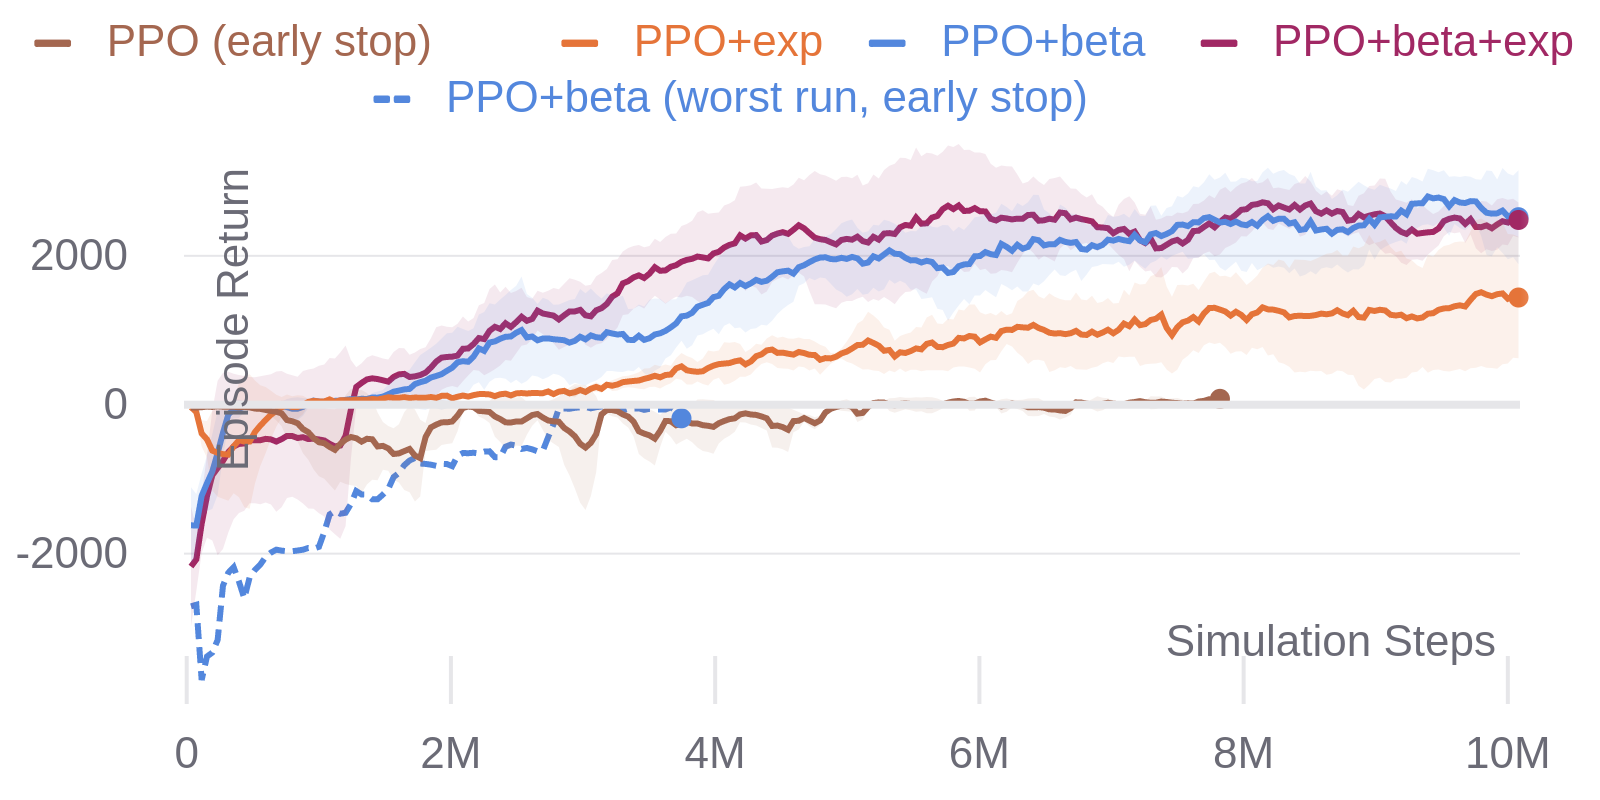
\includegraphics[width=\linewidth]{img/rl.png}
	\end{center}
	\vspace{-4ex}
	\caption{\textbf{Learning curves of RL experts }
		% Episode returns are averaged with a moving window of size 100. (removed because it's inaccurate, not 100 step, but 100 epoch, where one epoch=roullout+train)
		trained in CARLA Town 1-6.
		Solid lines show the mean and shaded areas show the standard deviation of episode returns across 3 seeds.
		The dashed line shows an outlier run that collapsed.}
	\vspace{-2ex}
	\label{fig:rl}
\end{figure}

\subsection{Performance of Experts}

\textbf{\textsf{Sample Efficiency:}}
To improve the sample efficiency of PPO, we propose to use BEV instead of camera images, Beta instead of Gaussian distributions, and the exploration loss in addition to the entropy loss.
Since the benefit of using a BEV representation is obvious, here we only ablate the Beta distribution and the exploration loss.
As shown in Fig.~\ref{fig:rl}, the baseline PPO with Gaussian distribution and entropy loss is trapped in a local minimum where staying still is the most rewarding strategy.
Leveraging the exploration loss, PPO+exp can be successfully trained despite relatively high variance and low sample efficiency.
The Beta distribution helps substantially, but without the exploration loss the training still collapsed in some cases due to insufficient exploration (cf. dashed blue line in Fig.~\ref{fig:rl}).
Our Roach (PPO+beta+exp) uses both Beta distribution and exploration loss to ensure stable and sample efficient training.
The training takes around 1.7M steps in each of the six CARLA servers, this accounts for 10M steps in total, which takes roughly a week on an AWS EC2 g4dn.4xlarge or 4 days on a 2080 Ti machine with 12 cores.


\textbf{\textsf{Driving Performance:}}
Table~\ref{table:expert_performance} compares different experts on the NoCrash-dense and on all 76 LeaderBoard routes under dynamic weather with busy traffic.
Our Autopilot is a strong baseline expert that achieves a higher success rate than the Autopilot used in LBC and DA-RB.
We evaluate three RL experts - 
(1) Roach, the proposed RL coach using Beta distribution and exploration prior.
(2) PPO+beta, the RL coach trained without using the exploration prior. 
(3) PPO+exp, the RL coach trained without using the Beta distribution.
In general, our RL experts achieve comparable success rates and higher driving scores than Autopilots because RL experts handle traffic lights in a better way (cf. Table~\ref{table:infraction}).
The two Autopilots often run red lights because they drive over-conservatively and wait too long at the junction, thus missing the green light.
Among RL experts, PPO+beta and Roach, the two RL experts using a Beta distribution, achieve the best performance, while the difference between both is not significant. PPO+exp performs slightly worse, but it still achieves better driving scores than our Autopilot. 


\begin{table}
	\setlength{\tabcolsep}{2.32pt}
	\centering
	\begin{tabular}{lccccc}
		\toprule
		Suc. Rate \% $\uparrow$
		& NCd-tt & NCd-tn  & NCd-nt & NCd-nn & LB-all  \\ 
		\cmidrule(lr){1-1}\cmidrule(lr){2-6}
		PPO+exp & $86 \pm 6$ & $86 \pm 6$ & $79 \pm 6$ & $77 \pm 5$ & $67\pm3$  \\
		PPO+beta & $\mathbf{95} \pm 3$ & $\mathbf{95} \pm 3$ & $83 \pm 5$ & $\mathbf{87} \pm 6$ & $72 \pm 5$  \\
		Roach & $91 \pm 4$ & $90 \pm 7$ & $\mathbf{83} \pm 3$ & $83 \pm 3$ & $72 \pm 6$  \\
		% Roach &
		% $91 \pm 4$ & $89 \pm 5$ & $\mathbf{90} \pm 3$ & $\mathbf{89} \pm 3$ & $69 \pm 4$ \\
		\cmidrule(lr){1-1}\cmidrule(lr){2-6}
		AP (ours) & 
		$\mathbf{95} \pm 3$ & $\mathbf{95} \pm 3$ & $83 \pm 5$ & $81 \pm 2$ & $\mathbf{75} \pm 8$ \\
		AP-lbc \cite{chen2020learning}
		& $86 \pm 3$ & $83 \pm 6$ & $60 \pm 3$ & $59 \pm 8$ & N/A \\
		AP-darb \cite{prakash2020exploring}
		& $71 \pm 4$ & $72 \pm 3$ & $41 \pm 2$ & $43 \pm 2$ & N/A \\
		% \bottomrule
		\toprule
		Dri. Score \% $\uparrow$
		& NCd-tt & NCd-tn  & NCd-nt & NCd-nn & LB-all  \\ 
		\cmidrule(lr){1-1}\cmidrule(lr){2-6}
		PPO+exp & $92 \pm 2$ & $92 \pm 2$ & $88 \pm 3$ & $86 \pm 1$ & $ 83\pm0$  \\
		PPO+beta & $\mathbf{98} \pm 2$ & $\mathbf{98} \pm 2$ & $90 \pm 3$ & $\mathbf{92} \pm 2$ & $\mathbf{86} \pm 2$  \\
		Roach & $95 \pm 2$ & $95 \pm 3$ & $\mathbf{91} \pm 3$ & $90 \pm 2$ & $85 \pm 3$  \\
		% Roach
		% & $93 \pm 1$ & $91 \pm 1$ & $91 \pm 4$ & $91 \pm 4$
		% & $79 \pm 1$ \\
		\cmidrule(lr){1-1}\cmidrule(lr){2-6}
		AP (ours)
		& $86 \pm 2$ & $86 \pm 2$ & $70 \pm 2$ & $70 \pm 1$
		& $78 \pm 3$ \\
		\bottomrule
	\end{tabular}
	\vspace{-1ex}
	\caption{\textbf{Success rate and driving score of experts.} Mean and standard deviation over 3 evaluation seeds. 
	NCd: NoCrash-dense. 
	tt: train town \& weather. 
	tn: train town \& new weather. 
	nt: new town \& train weather. 
	nn: new town \& weather. 
	LB-all: all 76 routes of LeaderBoard with dynamic weather. 
	AP: CARLA Autopilot. 
	For RL experts the best checkpoint among all training seeds and runs is used.}
	\label{table:expert_performance}
	\vspace{-2ex}
\end{table}



\subsection{Performance of IL Agents}
The performance of an IL agent is limited by the performance of the expert it is imitating.
If the expert performs poorly, it is not sensible to compare IL agents imitating that expert.
As shown in Table~\ref{table:expert_performance}, this issue is evident in the NoCrash new town with dense traffic, where Autopilots do not perform well. 
To ensure a high performance upper-bound and hence a fair comparison, we conduct ablation studies (Fig.~\ref{fig:score_eu_lb_tt_tn} and Table~\ref{table:infraction}) under the busy traffic setting such that our Autopilot can achieve a driving score of 80\% and a success rate of 90\%. 
In order to compare with the state-of-the-art, the best model from the ablation studies is still evaluated on NoCrash with dense traffic in Table~\ref{table:sucess_rate_nc_dense}.


The input measurement vector $\mathbf{m}_\text{IL}$ is different for the NoCrash and for the LeaderBoard. For NoCrash, $\mathbf{m}_\text{IL}$ is just the speed.
For the LeaderBoard, $\mathbf{m}_\text{IL}$ contains additionally a 2D vector pointing to the next desired waypoint.
This vector is computed from noisy GPS measurements and the desired route is specified as sparse GPS locations.
The LeaderBoard instruction suggests that it is used to disambiguate situations where the semantics of left and right are not clear due to the complexity of the considered map.
% As suggested by the LeaderBoard instruction, it is used to disambiguate situations where semantics of left and right are not clear due to the complexity of the considered map.
\begin{figure*}[t]
	\centering
	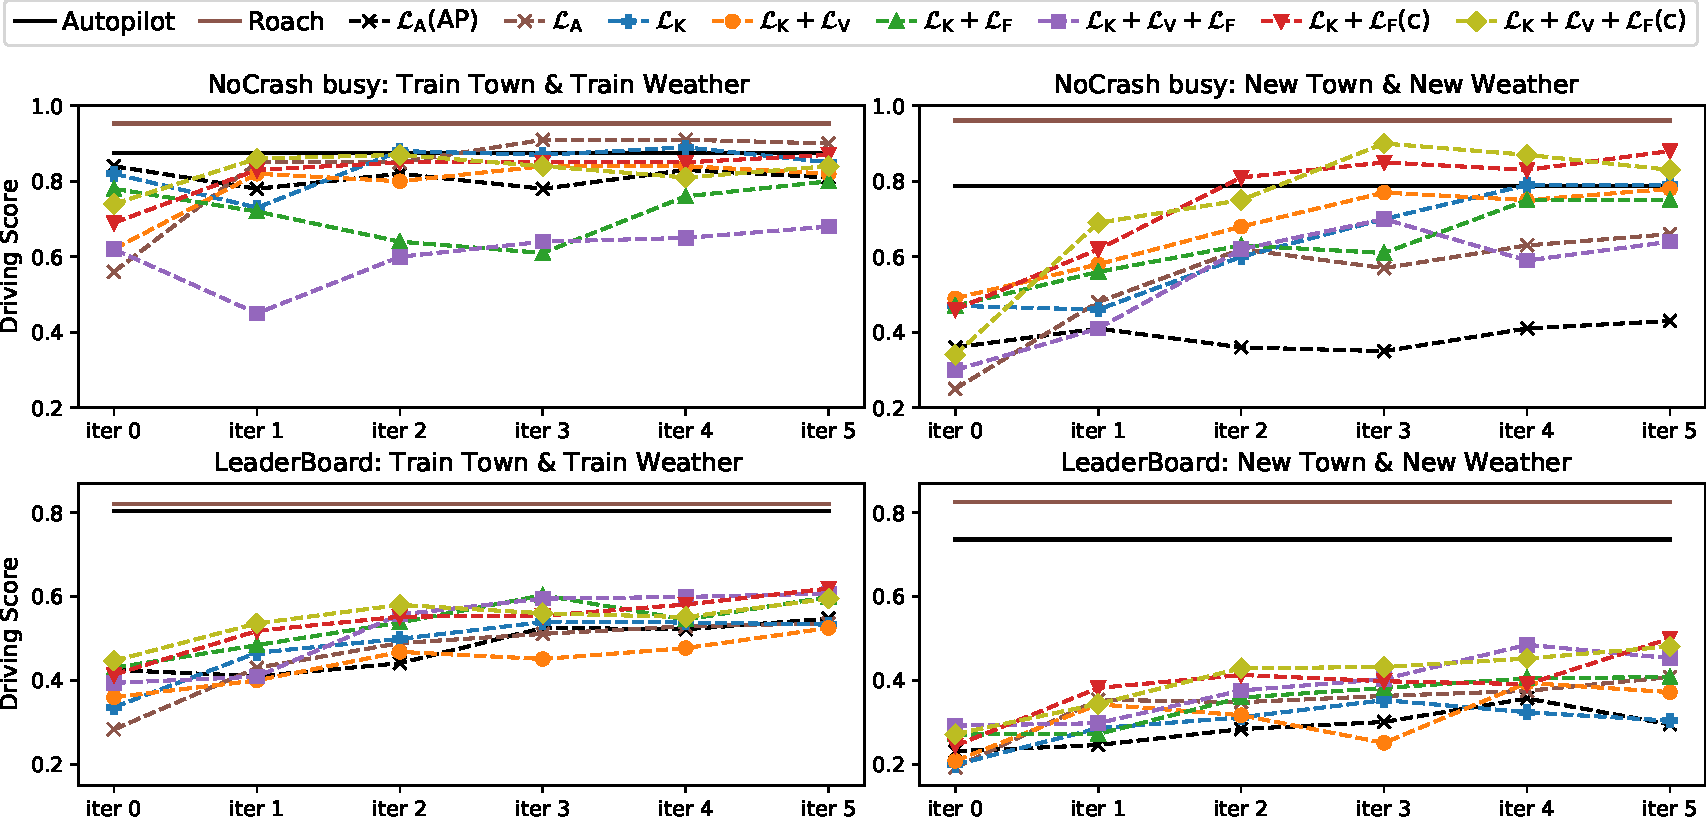
\includegraphics[width=0.99\textwidth]{img/score_eu_lb_tt_tn.pdf}
	\vspace{-1ex}
	\caption{\textbf{Driving score of experts and IL agents.} All IL agents (dashed lines) are supervised by Roach except for $\mathcal{L}_\text{A}(\text{AP})$, which is supervised by our Autopilot. For IL agents at the 5th iteration on NoCrash and all experts, results are reported as the mean over 3 evaluation seeds. Others are evaluated with one seed. The offline Leaderboard benchmark is used here.}
	\vspace{-1.5ex}
	\label{fig:score_eu_lb_tt_tn}
\end{figure*}


% table:sucess_rate_nc_dense
\begin{table}
	\setlength{\tabcolsep}{2.67pt}
	\centering
	\begin{tabular}{lccccc}
		\toprule
		Success Rate \% $\uparrow$
		&  NCd-tt & NCd-tn  & NCd-nt & NCd-nn  \\ 
		\cmidrule(lr){1-1}\cmidrule(lr){2-5}
		% LBC \cite{chen2020learning} ($\leq$ 0.9.5)  & 
		% $95 \pm 2$ & $97 \pm 2$ & $89 \pm 1$ & $85 \pm 1$ \\
		LBC \cite{chen2020learning} (0.9.6) & 
		$71 \pm 5$ & $63 \pm 3$ & $51 \pm 3$ & $39 \pm 6$ \\
		% LBC \cite{chen2020learning} (0.9.6, repo) & 
		% $70 \pm 5$ & $63 \pm 2$ & $46 \pm 4$ & $33 \pm 10$ \\
		% MaRLn \cite{toromanoff2020end} (0.9.6) & 
		% $ 70 $ & $ 26 $ & $ 42 $ & $ 18 $ \\
		SAM \cite{zhao2021sam} (0.8.4) & 
		$54 \pm 3$ & $47 \pm 5$ & $29 \pm 3$ & $29 \pm 2$ \\
		LSD \cite{ohn2020learning} (0.8.4) & 
		N/A & N/A & $30 \pm 4$ & $32 \pm 3$ \\
		DA-RB\textsuperscript{+}(E) \cite{prakash2020exploring} & 
		$66 \pm 5$ & $56 \pm 1$ & $36 \pm 3$ & $35 \pm 2$ \\
		DA-RB\textsuperscript{+} \cite{prakash2020exploring} (0.8.4)  & 
		$62 \pm 1$ & $60 \pm 1$ & $34 \pm 2$ & $25 \pm 1$ \\
		Our baseline, $\mathcal{L}_\text{A}\text{(AP)}$ & 
		$\mathbf{88} \pm 4$ & $29 \pm 3$ & $32 \pm 11$ & $28 \pm 4$ \\
		Our best, $\mathcal{L}_\text{K}+\mathcal{L}_\text{F}(\text{c})$ & 
		$86 \pm 5$ & $\mathbf{82} \pm 2$ & $\mathbf{78} \pm 5$ & $\mathbf{78} \pm 0$ \\
		% DA-RB\textsuperscript{+}Roach(K,V,F,c) & 
		% $ \pm $ & $ \pm $ & $ \pm $ & $ \pm $ \\
		\bottomrule
	\end{tabular}
	\vspace{-1ex}
	\caption{\textbf{Success rate of camera-based end-to-end IL agents on NoCrash-dense.} Mean and standard deviation over 3 seeds. Our models are from DAGGER iteration 5. For DA-RB, + means triangular perturbations are added to the off-policy dataset, (E) means ensemble of all iterations.}
	\label{table:sucess_rate_nc_dense}
	\vspace{-2ex}
\end{table}
% table:infraction
\begin{table*}
	\setlength{\tabcolsep}{3.8pt}
	\centering
	\begin{tabular}{lccccccccc} 
		\toprule
		& \begin{tabular}{@{}c@{}}Success \\ rate \end{tabular} 
		& \begin{tabular}{@{}c@{}}Driving \\ score \end{tabular} 
		& \begin{tabular}{@{}c@{}}Route \\ compl. \end{tabular} 
		& \begin{tabular}{@{}c@{}}Infrac. \\ penalty \end{tabular} 
		& \begin{tabular}{@{}c@{}}Collision \\ others \end{tabular} 
		& \begin{tabular}{@{}c@{}}Collision \\ pedestrian \end{tabular} 
		& \begin{tabular}{@{}c@{}}Collision \\ vehicle \end{tabular}  
		& \begin{tabular}{@{}c@{}}Red light \\ infraction \end{tabular}  
		& \begin{tabular}{@{}c@{}}Agent \\ blocked \end{tabular}  \\
		\cmidrule(lr){1-1}\cmidrule(lr){2-5}\cmidrule(lr){6-10}
		iter 5
		& \%, $\uparrow$
		& \%, $\uparrow$
		& \%, $\uparrow$
		& \%, $\uparrow$
		& \#/Km, $\downarrow$
		& \#/Km, $\downarrow$
		& \#/Km, $\downarrow$
		& \#/Km, $\downarrow$
		& \#/Km, $\downarrow$
		\\
		\cmidrule(lr){1-1}\cmidrule(lr){2-5}\cmidrule(lr){6-10}
		% $\mathcal{L}_\text{A}$
		% & $\pm$ & $\pm$ & $\pm$ & $\pm$ 
		% & $\pm$ & $\pm$ & $\pm$ & $\pm$ & $\pm$ \\
		$\mathcal{L}_\mathrm{A}(\text{AP})$
		& $31 \pm 7$ & $43 \pm 2$ & $62 \pm 6$ & $77 \pm 4$ 
		& $0.54 \pm 0.53$ & $\mathbf{0}\pm0$ & $0.63 \pm 0.50$ & $3.33 \pm 0.58$ & $19.4\pm 14.4$ \\
		$\mathcal{L}_\text{A}$
		& $57\pm7$ & $66\pm3$ & $84\pm3$ & $76\pm1$ 
		& $2.07\pm1.37$ & $\mathbf{0}\pm0$ & $1.36\pm1.10$ & $1.4\pm0.2$ & $2.82\pm1.45$ \\
		$\mathcal{L}_\text{K}$
		& $74\pm3$ & $79\pm0$ & $91\pm2$ & $86\pm1$ 
		& $0.50\pm0.25$ & $\mathbf{0}\pm0$ & $0.53\pm0.18$ & $0.68\pm0.08$ & $3.39\pm0.20$ \\
		% $\mathcal{L}_\text{K}+\mathcal{L}_\text{V}$
		% & $71\pm9$ & $78\pm3$ & $91\pm1$ & $85\pm3$ 
		% & $0.55\pm0.22$ & $0.11\pm0.06$ & $0.34\pm0.31$ & $0.72\pm0.09$ & $1.14\pm0.10$ \\
		% $\mathcal{L}_\text{K}+\mathcal{L}_\text{F}$
		% & $62\pm2$ & $75\pm1$ & $85\pm0$ & $87\pm2$ 
		% & $0.79\pm0.61$ & $0.03\pm0.05$ & $0.73\pm0.16$ & $0.63\pm0.02$ & $2.04\pm1.33$ \\
		$\mathcal{L}_\text{K}+\mathcal{L}_\text{F}(\text{c})$
		& $\mathbf{87} \pm 5$ & $\mathbf{88} \pm 3$ & $\mathbf{96} \pm 0$ & $\mathbf{91} \pm 3$ 
		& $\mathbf{0.08} \pm 0.04$ & $0.01 \pm 0.02$ & $\mathbf{0.23} \pm 0.08$ & $\mathbf{0.61} \pm 0.23$ & $\mathbf{0.84} \pm 0.04$ \\
		\cmidrule(lr){1-1}\cmidrule(lr){2-5}\cmidrule(lr){6-10}
		Roach
		& $95 \pm 2$ & $96 \pm 3$ & $100 \pm 0$ & $96 \pm 3$ 
		& $0 \pm 0$ & $0.11 \pm 0.07$ & $0.04 \pm 0.05$ & $0.16 \pm 0.20$ & $0 \pm 0$ \\
		Autopilot
		& $91 \pm 1$ & $79 \pm 2$ & $98 \pm 1$ & $80 \pm 2$ 
		& $0 \pm 0$ & $0 \pm 0$ & $0.18 \pm 0.08$ & $1.93 \pm 0.23$ & $0.18 \pm 0.08$\\
		\bottomrule
	\end{tabular}
	\vspace{-1ex}
	\caption{\textbf{Driving performance and infraction analysis of IL agents on NoCrash-busy, new town \& new weather.} Mean and standard deviation over 3 evaluation seeds.}
	\vspace{-2.5ex}
	\label{table:infraction}
\end{table*}

\vspace{1ex}\noindent{\bf Ablation:}
Fig.~\ref{fig:score_eu_lb_tt_tn} shows driving scores of experts and IL agents at each DAGGER iteration on NoCrash and offline LeaderBoard with busy traffic.
The baseline $\mathcal{L}_\text{A}(\text{AP})$ is our implementation of DA-RB\textsuperscript{+} supervised by our Autopilot. 
Given our improved Autopilot, it is expected that $\mathcal{L}_\text{A}(\text{AP})$ can achieve higher success rates than those reported in the DA-RB paper, but this is not observed in Table~\ref{table:sucess_rate_nc_dense}.
The large performance gap between the Autopilot and $\mathcal{L}_\text{A}(\text{AP})$ (cf. Fig.~\ref{fig:score_eu_lb_tt_tn}), especially while generalizing to a new town and new weather, indicates the limitation of this baseline.


By replacing the Autopilot with Roach, $\mathcal{L}_\text{A}$ performs better overall than $\mathcal{L}_\text{A}(\text{AP})$.
Further learning from the action distribution, $\mathcal{L}_\text{K}$ generalizes better than $\mathcal{L}_\text{A}$ on the NoCrash but not on the offline LeaderBoard.
Feature matching only helps when $\mathbf{j}_\text{IL}$ is provided with the necessary information needed to reproduce $\mathbf{j}_\text{RL}$.
In our case, $\mathbf{j}_\text{RL}$ contains navigational information as the desired route is rendered in the BEV input.
For the LeaderBoard, navigational information is partially encoded in $\mathbf{m}_\text{IL}$, which includes the vector to the next desired waypoint, so better performance is observed by using $\mathcal{L}_\text{F}$.
But for NoCrash this information is missing as $\mathbf{m}_\text{IL}$ is just the speed, hence it is impractical for $\mathbf{j}_\text{IL}$ to mimic $\mathbf{j}_\text{RL}$ and this causes the inferior performance of $\mathcal{L}_\text{K}+\mathcal{L}_\text{F}$ and $\mathcal{L}_\text{K}+\mathcal{L}_\text{F}+\mathcal{L}_\text{V}$.
To confirm this hypothesis, we evaluate a single-branch network architecture where the measurement vector $\mathbf{m}_\text{IL}$ is augmented by the command encoded as a one-hot vector.
Using feature matching with this architecture, $\mathcal{L}_\text{K}+\mathcal{L}_\text{F}(\text{c})$ and $\mathcal{L}_\text{K}+\mathcal{L}_\text{V}+\mathcal{L}_\text{F}(\text{c})$ achieve the best driving score among IL agents in the NoCrash new town \& weather generalization test, even outperforming the Autopilot.

Using value supervision in addition to feature matching helps the DAGGER process to converge faster as shown by $\mathcal{L}_\text{K}+\mathcal{L}_\text{V}+\mathcal{L}_\text{F}$ and $\mathcal{L}_\text{K}+\mathcal{L}_\text{V}+\mathcal{L}_\text{F}(\text{c})$.
However, without feature matching, using value supervision alone $\mathcal{L}_\text{K}+\mathcal{L}_\text{V}$ does not demonstrate superior performance.
This indicates a potential synergy between feature matching and value estimation.
Intuitively, the latent feature of Roach encodes the information needed for value estimation, hence mimicking this feature should help to predict the value,
while value estimation could help to regularize feature matching.

% In general, using value supervision does not have a significant effect on the performance, presumably because estimating the long-term reward from a single camera image is too difficult and thus not informative.
% However, on the LeaderBoard is achieved by using $\mathcal{L}_\text{V}$ together with $\mathcal{L}_\text{F}$, which indicates a potential synergy between feature mimicking and value estimation.
% Intuitively, the latent feature of Roach encodes information needed for value estimation, hence mimicking this feature should also help to predict value.
% And value estimation as a side task could help to regularize feature matching.

\vspace{1ex}\noindent{\bf Comparison with the State-of-the-art:}
In Table~\ref{table:sucess_rate_nc_dense} we compare the baseline $\mathcal{L}_\text{A}(\text{AP})$ and our best performing agent $\mathcal{L}_\text{K}+\mathcal{L}_\text{F}(\text{c})$ with the state-of-the-art on the NoCrash-dense benchmark.
Our $\mathcal{L}_\text{A}(\text{AP})$ performs comparably to DA-RB\textsuperscript{+} except when generalizing to the new weather, where there is an incorrect rendering of after-rain puddles on CARLA 0.9.11 (see supplement for visualizations).%, which is hard in CARLA 0.9.11 due to a rendering issue of reflections from after-rain puddles (see supplement for visualizations).
This issue does not affect our best method $\mathcal{L}_\text{K}+\mathcal{L}_\text{F}(\text{c})$ due to the stronger supervision of Roach. 
By mimicking the weather-agnostic Roach, the performance of our IL agent drops by less than $10\%$ while generalizing to the new town and weather.
Hence if the Autopilot is considered the performance upper-bound, it is fair to claim our approach saturates the NoCrash benchmark.
However, as shown in Fig.~\ref{fig:score_eu_lb_tt_tn}, there is still space for improvement on NoCrash compared to Roach and the performance gap on the offline LeaderBoard highlights the importance of this new benchmark.

\vspace{1ex}\noindent{\bf Performance and Infraction Analysis:}
Table~\ref{table:infraction} provides the detailed performance and infraction analysis on the NoCrash benchmark with busy traffic in the new town \& weather setting.
Most notably, the extremely high ``Agent blocked'' of our baseline $\mathcal{L}_\text{A}(\text{AP})$ is due to reflections from after-rain puddles.
This problem is largely alleviated by imitating Roach, which drives more naturally, and $\mathcal{L}_\text{A}$ shows an absolute improvement of $23\%$ in terms of driving score.
In other words this is the gain achieved by using a better expert, but the same imitation learning approach. 
% Learning from the action distribution of Roach leads to another $13\%$ improvement by reducing collisions.
Further using the improved supervision from soft targets and latent features results in our best model $\mathcal{L}_\text{K}+\mathcal{L}_\text{F}(\text{c})$, which demonstrates another $22\%$ absolute improvement.
% And the best performance is achieved by $\mathcal{L}_\text{K}+\mathcal{L}_\text{F}(\text{c})$ that combines the idea of learning from soft targets and latent features, which results in another $9\%$ improvement.
By handling red lights in a better way, this agent achieves $88\%$, an expert-level driving score, using a single camera image as input.



 